\documentclass{article}
\usepackage[final]{colm2025_conference}

\usepackage{microtype}
\usepackage{hyperref}
\usepackage{url}
\usepackage{booktabs}
\usepackage{graphicx}
\usepackage{amsmath}
\usepackage{enumitem}
\usepackage{amssymb}
\usepackage{textcomp}

\title{CRISP: Coach-Regulated Iterative Solver Pairing\\for Mathematical Problem Solving}

\author{Alexander Baumgartner \& Sahil Agrawal \\
University of Chicago \\
\texttt{\{abaumgartner, sahilagr\}@uchicago.edu} \\
\And
Project Mentor: Qirun Dai \\
University of Chicago \\
\texttt{qirundai@uchicago.edu} \\
}

\newcommand{\fix}{\marginpar{FIX}}
\newcommand{\new}{\marginpar{NEW}}

\begin{document}

\maketitle

\begin{abstract}
Single-agent reinforcement learning with verifiable rewards (RLVR) is limited by static training data that wastes compute on mastered or impossible problems, and by sparse binary rewards that cannot distinguish sound reasoning from lucky pattern-matching. We introduce \textbf{CRISP} (Coach-Regulated Iterative Solver Pairing), a three-agent system in which an adaptive coach (Qwen3-14B) generates problems targeting the 50\% solve-rate frontier, where GRPO gradients are maximized, and two independently-trained players (Qwen3-4B) discuss only when they disagree, following Mazur's Peer Instruction principle. Each agent trains in its own reward universe with independent EMA-normalized advantages, preventing gradient instability from pooled multi-agent rewards. Over 44 iterations on 4$\times$H200 GPUs, the coach's difficulty calibration drives accuracy from 97\% during warmup to oscillating around the optimal 50\% frontier, while peer discussions increase from 0 to 4--6 per batch, confirming that the adaptive curriculum and social learning mechanisms reinforce each other.
\end{abstract}

\section{Introduction}

Reinforcement learning with verifiable rewards (RLVR) has become the dominant paradigm for training mathematical reasoning in LLMs since \citet{guo2025deepseek} demonstrated that GRPO with binary correctness rewards produces emergent chain-of-thought reasoning. The recipe is simple: generate rollouts, verify against ground truth, and reinforce correct solutions. However, single-agent RLVR on a fixed dataset exposes three failure modes. \emph{Sparse signal:} binary correctness treats pattern-matching and rigorous proofs identically, providing no signal about reasoning quality. \emph{Static data:} problems that are too easy or too hard produce zero-variance GRPO groups with zero gradient. In our baseline, nearly every group was zero-variance with $G\!=\!4$ rollouts until we increased to $G\!=\!8$ with dynamic filtering \citep{yu2025dapo}. \emph{Data dependence:} RLVR requires large verified problem sets that many domains lack.

Recent work addresses these failures individually: CPM\"{o}bius \citep{li2026cpmobius} and R-Zero \citep{huang2025rzero} replace static datasets with coach-generated problems; MAPoRL \citep{park2025maporl} adds multi-agent discussion rewards; Dr.~MAS \citep{zhu2025drmas} introduces agent-wise advantage normalization. However, no existing system combines adaptive curriculum generation with social learning in a single training loop. The two mechanisms are potentially synergistic: a coach that targets the difficulty frontier should naturally produce problems where agents disagree, and disagreement outcomes can inform the coach's reward, but this interaction has not been explored.

We propose \textbf{CRISP} (Coach-Regulated Iterative Solver Pairing), a three-agent system that closes this loop. An adaptive coach (Qwen3-14B) generates problems targeting 50\% solve rate, where GRPO gradients are maximized \citep{pcl2025}. Two independently-trained players (Qwen3-4B) solve each problem and discuss only when they disagree, following Mazur's Peer Instruction \citep{crouch2001peer}. Discussion outcomes feed back into the coach's reward, creating a cycle: harder problems produce more disagreements, productive disagreements reward the coach, and the coach learns to generate problems in the zone where both curriculum and discussion are most effective. Each agent trains in its own reward universe with independent EMA-normalized advantages, preventing the gradient instability that arises from pooling multi-agent rewards \citep{zhu2025drmas}.

Building this system also revealed that multi-agent RLVR is substantially harder to engineer than the algorithmic description suggests. We document five coach failure modes, several optimizer pathologies, and the GPU memory engineering required to co-train three models on 4$\times$H200 GPUs. These lessons generalize to other multi-agent RL systems for LLMs.

\paragraph{Contributions.}
(1)~The first RLVR system integrating adaptive coach-player co-evolution with peer discussion in a single training loop, where discussion outcomes directly inform the coach's reward.
(2)~A per-problem coach reward (uncertainty targeting + discussion productivity $-$ repetition penalty) replacing batch-level signals, with coach self-solve for ground truth.
(3)~Independent per-player training with agent-wise advantage normalization, preventing gradient instability from pooled multi-agent rewards.
(4)~A characterization of multi-agent RLVR failure modes and the engineering required for a working deployment.


\section{Related Work}

\paragraph{Single-agent RLVR.} DeepSeek-R1 \citep{guo2025deepseek} established that GRPO with binary rewards produces emergent reasoning without SFT. DAPO \citep{yu2025dapo} improved training stability with dynamic sampling and clip-higher; DCPO \citep{xu2025dcpo} introduced token-adaptive clipping. Our baseline replicates this recipe at smaller scale. These methods all train a single agent on a fixed dataset; CRISP extends the paradigm by making both the data source and the learning process adaptive and social.

\paragraph{Coach-player co-evolution.} CPM\"{o}bius \citep{li2026cpmobius} introduced coach-player co-evolution for data-free RL, rewarding the coach via a batch-level difficulty delta $\Delta_t$. R-Zero \citep{huang2025rzero} refined this with uncertainty targeting near 50\% solve rate and BLEU-based repetition penalties. R-Zero also showed that player majority vote as pseudo-ground-truth degrades from 79\% to 63\% accuracy on harder problems. CRISP builds on both: we adopt uncertainty targeting as our core coach signal, upgrade BLEU to MiniLM embedding similarity for repetition detection, replace batch-level $\Delta_t$ with a per-problem composite reward, and substitute coach self-solve for majority-vote ground truth. Crucially, neither CPM\"{o}bius nor R-Zero incorporates multi-agent discussion; the coach generates problems but agents solve in isolation.

\paragraph{Multi-agent LLM collaboration.} MARTI \citep{chen2025marti} provided the multi-agent RLVR infrastructure (DeepSpeed/vLLM integration, multi-agent rollout generation) on which CRISP's codebase builds. MAPoRL \citep{park2025maporl} showed that co-training LLMs with discussion rewards yields genuine collaboration, reporting a 9.5\% boost from a persuadability reward. \citet{zhang2025lazy} identified lazy-agent collapse where one agent dominates. We adopt MAPoRL's discussion protocol but simplify their reward from four parameters to three terms with segment-level credit assignment, and mitigate lazy-agent collapse with distinct player prompts/temperatures and JS-divergence regularization. However, neither MARTI nor MAPoRL incorporates an adaptive coach; both use fixed datasets. CRISP is the first system to combine coach-generated problems with inter-agent discussion, enabling the coach to reward discussion-producing problems directly.

\paragraph{Advantage normalization.} Dr.~MAS \citep{zhu2025drmas} demonstrated that agent-wise advantage normalization prevents gradient instability from pooling agents with different reward distributions, replacing centralized MAGRPO-style pooling \citep{liu2025magrpo}. We adopt this principle: each player maintains independent EMA trackers. PCL \citep{pcl2025} provides the theoretical grounding for our 50\% difficulty target, proving that GRPO gradient magnitude is maximized at this solve rate.


\section{Methods}

We describe the CRISP pipeline in its final form, then summarize the experimental conditions and evaluation protocol. Appendix~\ref{sec:evolution} describes the iterative design process that led to this architecture, including the failure modes that motivated each change.

\subsection{Overview}

The CRISP pipeline operates in seven steps per training iteration (Figure~\ref{fig:pipeline}):

\begin{figure}[t]
    \centering
    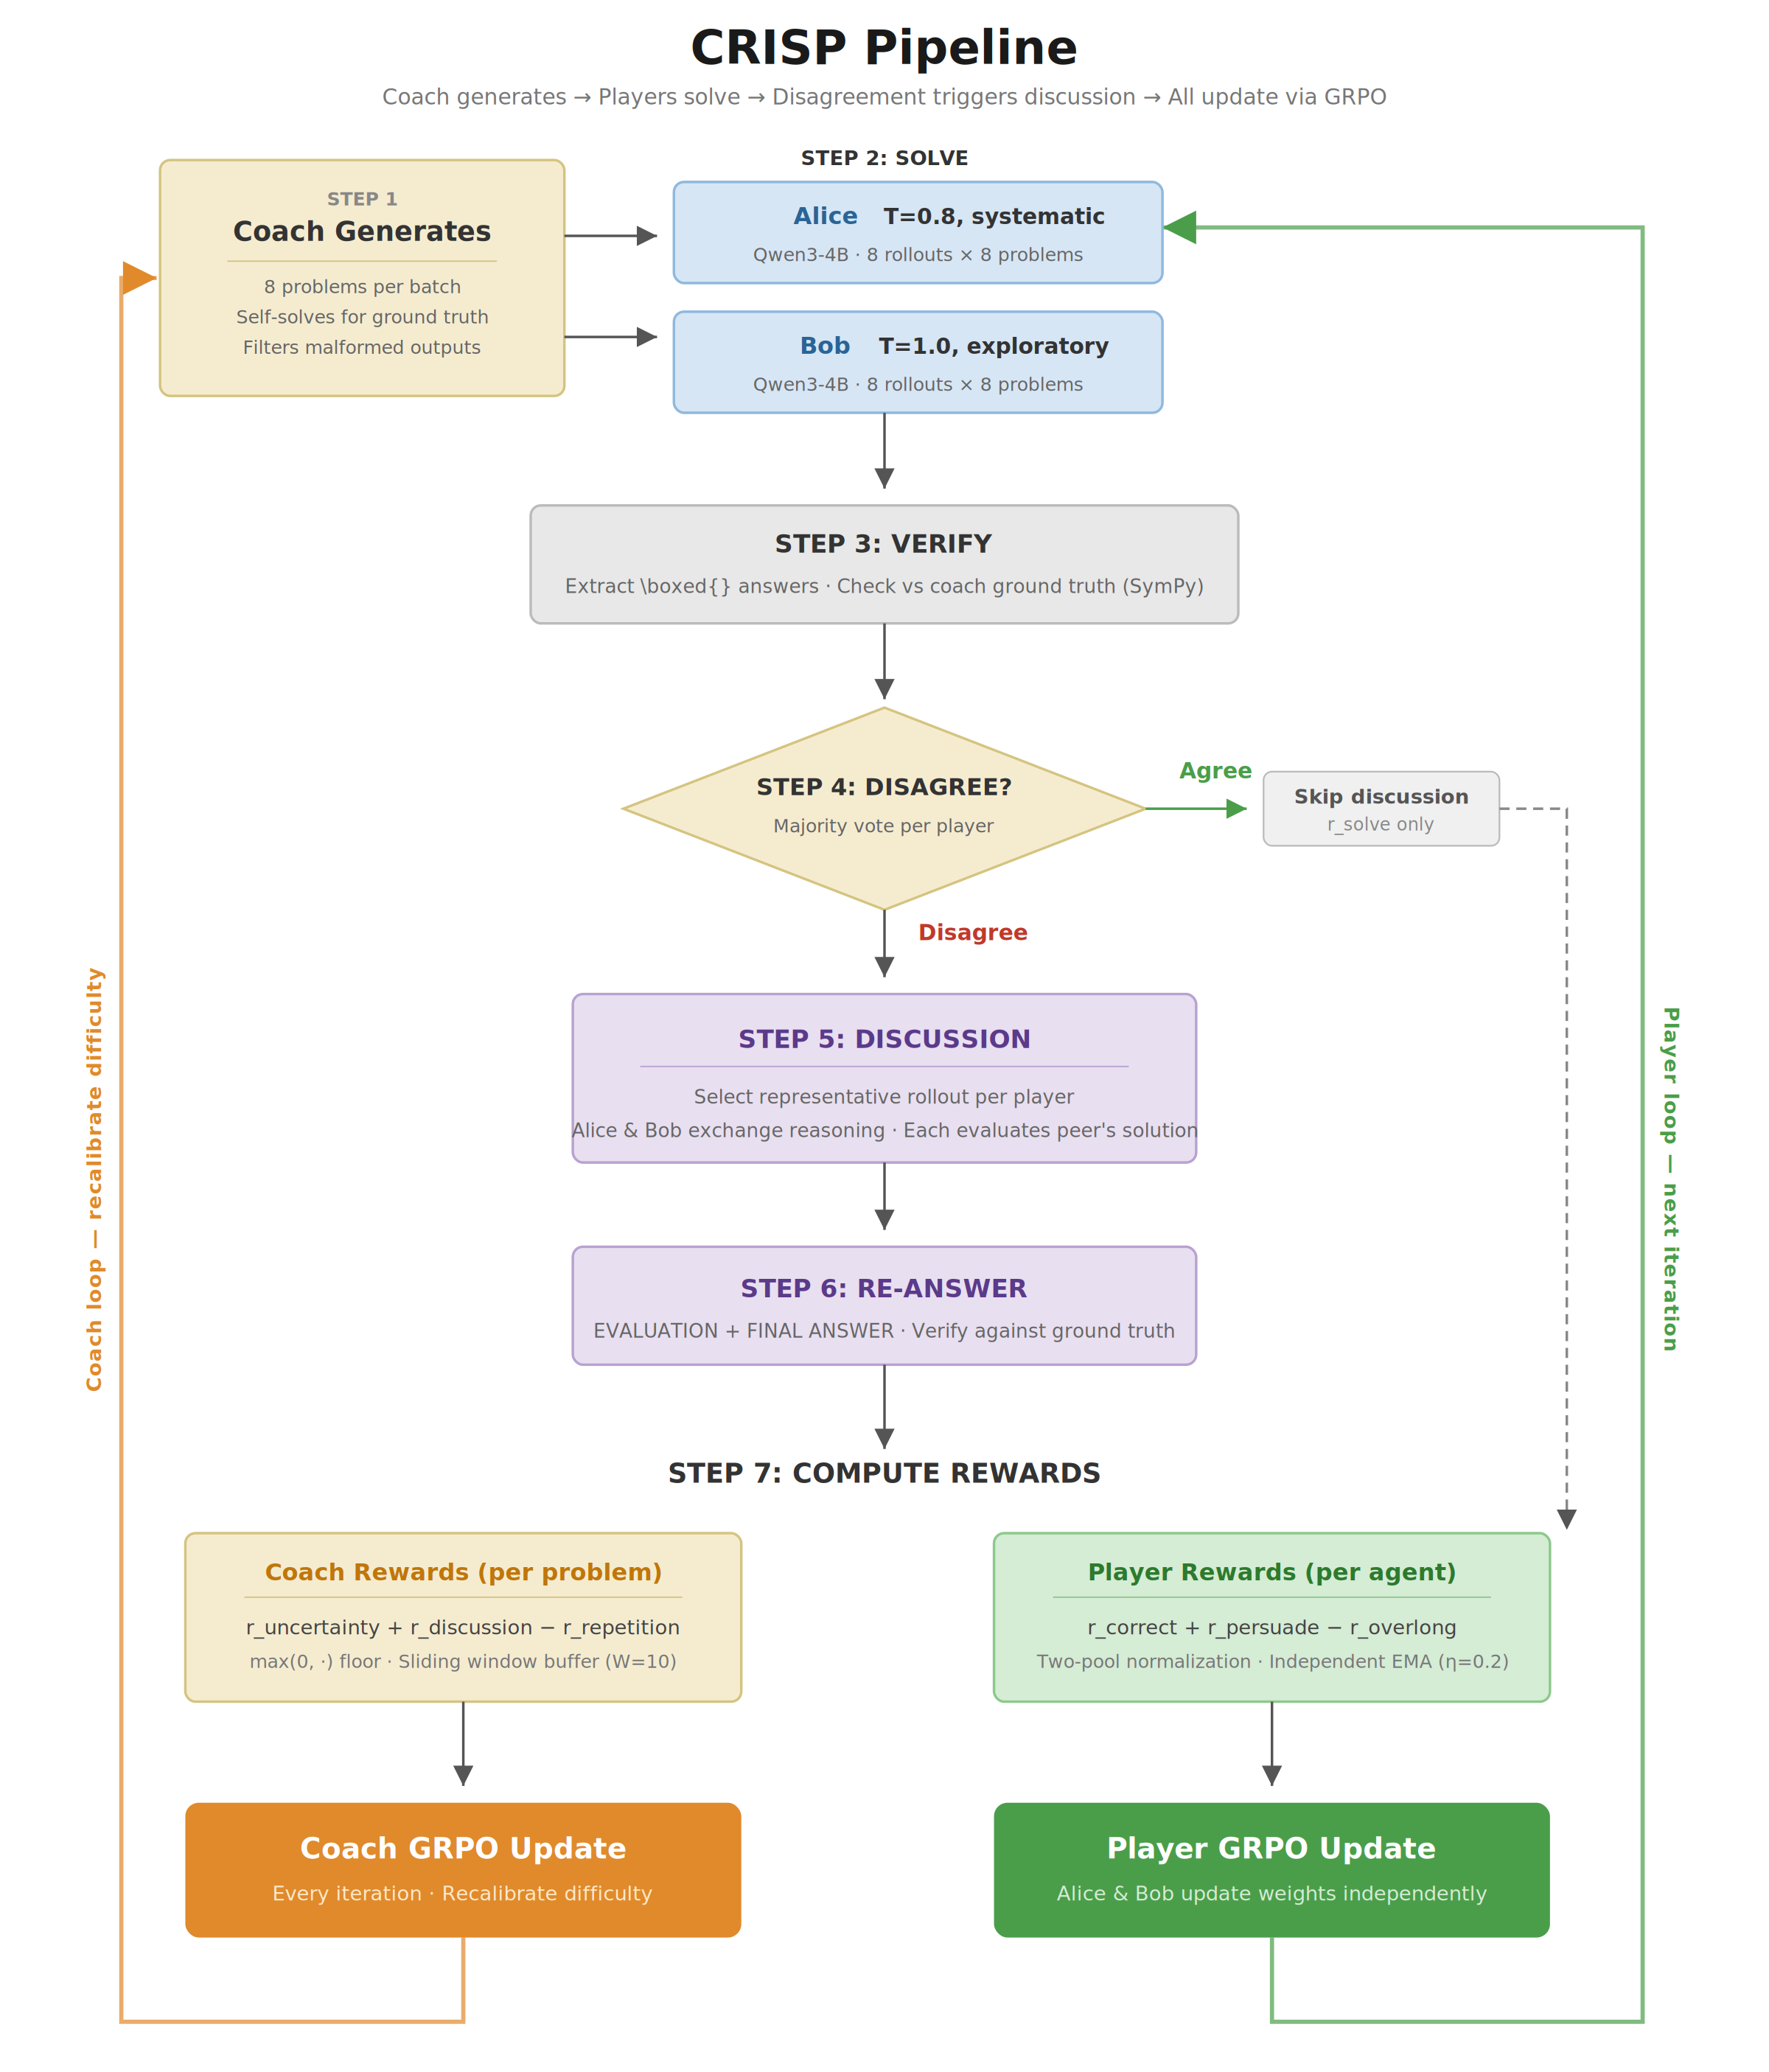
\includegraphics[width=\linewidth]{pipeline.png}
    \caption{The CRISP pipeline. The coach generates problems and self-solves for ground truth. Both players solve independently; if they disagree, they discuss. Rewards flow back to both players (correctness + persuader bonus) and the coach (uncertainty + discussion productivity $-$ repetition).}
    \label{fig:pipeline}
\end{figure}

\begin{enumerate}[leftmargin=*,itemsep=1pt]
    \item \textbf{Coach generates.} The coach produces 8 problems per batch, self-solves each for ground truth using \texttt{/think} mode, and filters malformed outputs.
    \item \textbf{Players solve.} Alice ($T\!=\!0.8$, systematic) and Bob ($T\!=\!1.0$, exploratory) each generate $G\!=\!8$ rollouts per problem independently. A shared vLLM engine serves both players via sequential weight synchronization.
    \item \textbf{Verify.} We extract \texttt{\textbackslash boxed\{\}} answers from each rollout and check against the coach's ground truth using SymPy semantic comparison.
    \item \textbf{Disagreement check.} We compute a majority-vote answer per player. If both players agree, the problem skips discussion and proceeds directly to GRPO. If they disagree, it enters Step~5.
    \item \textbf{Discussion.} Alice and Bob exchange reasoning: each receives a representative rollout from the other player and writes a structured response evaluating the peer's solution.
    \item \textbf{Re-answer.} Each player produces a post-discussion response with an evaluation of the peer's reasoning and a revised \texttt{\textbackslash boxed\{\}} answer, both verified against ground truth.
    \item \textbf{Compute rewards and update.} Player and coach rewards are computed (Sections~\ref{sec:coach_reward}--\ref{sec:player_reward}). Each player updates independently via GRPO with agent-wise advantage normalization. The coach updates via GRPO every iteration.
\end{enumerate}

Figure~\ref{alg:crisp} formalizes this procedure.

\begin{figure}[t]
\small
\fbox{\parbox{0.96\linewidth}{
\textbf{Algorithm 1:} CRISP Training Loop (one iteration) \\[2pt]
\textbf{Input:} Coach $\pi_C$, players $\pi_A, \pi_B$, rollouts $G$, batch size $B$ \\[3pt]
1.\quad $\{(x_i, y_i^*)\}_{i=1}^{B} \leftarrow \text{CoachGenerate}(\pi_C, B)$ \hfill \textit{\% problems + ground truth} \\
2.\quad \textbf{for} each player $p \in \{A, B\}$ \textbf{do} \\
3.\quad \quad $\{r_{ij}^p\}_{j=1}^{G} \leftarrow \text{Rollouts}(\pi_p, x_i, G)$ for all $i$; verify against $y_i^*$ \\
4.\quad $\hat{p}_i \leftarrow (\hat{p}_i^A + \hat{p}_i^B) / 2$ \hfill \textit{\% combined solve rate} \\
5.\quad \textbf{for} each problem $x_i$ \textbf{do} \\
6.\quad \quad $a_i^A \leftarrow \text{MajVote}(\pi_A, x_i)$; \; $a_i^B \leftarrow \text{MajVote}(\pi_B, x_i)$ \\
7.\quad \quad \textbf{if} $a_i^A \neq a_i^B$ \textbf{then} \hfill \textit{\% disagreement $\rightarrow$ discussion} \\
8.\quad \quad \quad Exchange representative rollouts; each player re-answers \\
9.\quad \quad \quad Compute $r_{\text{persuade}}$ from answer flips \\
10.\; $r_{\text{coach}}(x_i) \leftarrow \max\!\big(0,\; r_{\text{unc}}(\hat{p}_i) + r_{\text{disc}}(x_i) - r_{\text{rep}}(x_i)\big)$ \\
11.\; $r_{\text{player}}^p(r_{ij}^p) \leftarrow r_{\text{correct}} + r_{\text{persuade}} - r_{\text{overlong}}$ \\
12.\; \textbf{for} each player $p \in \{A, B\}$ \textbf{do} \\
13.\; \quad Normalize advantages via $p$'s independent EMA tracker \\
14.\; \quad Update $\pi_p$ via GRPO with DCPO clipping \\
15.\; Update $\pi_C$ via GRPO on coach rewards
}}
\caption{The CRISP training procedure for one iteration. Steps 7--9 execute only for problems where players disagree. Each player is updated independently (steps 12--14) with agent-wise advantage normalization.}
\label{alg:crisp}
\end{figure}

\subsection{Models, Data, and Infrastructure}

\paragraph{Players.} Both Alice and Bob are Qwen3-4B-Instruct-2507, initialized from identical base weights but trained as independent DeepSpeed ZeRO-2 engines with separate optimizers. Alice ($T\!=\!0.8$) is prompted to solve step-by-step: ``define variables, set up equations, solve algebraically.'' Bob ($T\!=\!1.0$) is prompted to ``try multiple approaches, look for patterns and shortcuts.'' Without this differentiation, both players almost always agree, collapsing to single-agent behavior.

\paragraph{Coach.} Qwen3-14B serves as the coach. Qwen3-14B natively supports hybrid thinking/non-thinking modes: the coach generates each problem in \texttt{/no\_think} mode (fast, no chain-of-thought overhead) and self-solves in \texttt{/think} mode (deep reasoning), producing verified ground truth. This avoids the degradation of player majority vote as pseudo-labels documented in R-Zero.

\paragraph{Training data.} For fixed-dataset conditions, we use DAPO-17K. For adaptive conditions, the coach generates problems from scratch with a three-phase difficulty curriculum: Phase~1 (warmup, 5 iterations) anchors at AMC~10, Phase~2 (ramp, 75 iterations) targets AMC~12/early AIME, and Phase~3 uses pure accuracy-driven calibration targeting 40--60\% solve rate.

\paragraph{Infrastructure.} The system runs on 4 GPUs (H200, 141\,GB each): GPU~0 hosts a shared vLLM engine for both players (sequential weight sync, ${\sim}1$s per sync for the 4B model), GPU~1 hosts the coach vLLM engine, GPU~2 hosts both player DeepSpeed engines plus the reference model (parked on CPU except during forward passes), and GPU~3 hosts the coach DeepSpeed engine. Adam optimizer states are offloaded to CPU (${\sim}280$\,GB total for three models). Gradient checkpointing and chunked \texttt{lm\_head} computation (chunk size 1024) keep GPU~2 peak memory under 32\,GB despite hosting two independently-trained 4B models.

\subsection{Coach Reward}
\label{sec:coach_reward}

Having described the pipeline structure, we now define the reward functions that govern learning. The coach receives a per-problem composite reward:
\begin{equation}
    r_{\text{coach}}(x) = \max\!\big(0,\; r_{\text{uncertainty}} + r_{\text{discussion}} - r_{\text{repetition}}\big)
\end{equation}

The $\max(0, \cdot)$ floor prevents negative rewards from destabilizing GRPO, following R-Zero. Three short-circuit penalties handle degenerate cases: unsolvable by coach ($-0.5$), too hard for all players ($-0.2$), and too easy ($-0.3$, suppressed during warmup).

\paragraph{Uncertainty reward.} Both players attempt each problem with $G\!=\!8$ rollouts each, and we compute a combined solve rate $\hat{p}(x)$. The reward is $r_{\text{uncertainty}} = 1 - 2|\hat{p} - 0.5|$, peaking at $\hat{p} = 0.5$. PCL \citep{pcl2025} proved that GRPO gradient magnitude is maximized at 50\% success probability.

\paragraph{Discussion productivity bonus.} For problems where players disagreed and discussion occurred, the coach receives $\alpha = 0.3$ if the discussion resolved correctly; $\alpha/2$ for unresolved discussions (the problem was at least in the right difficulty zone). This per-problem signal directly incentivizes problems in the Mazur zone.

\paragraph{Repetition penalty.} Problems are encoded with a frozen MiniLM-L6-v2 encoder. The penalty has two components: an intra-batch term penalizing similarity among problems within the current batch, and a cross-batch term using a sliding window buffer of the last $W\!=\!10$ batches. Both use cosine similarity ($\tau = 0.85$) with penalty proportional to cluster size ($\lambda = 2.5$). The cross-batch component addresses the ``local diversity illusion'' identified by R-Diverse \citep{rdiverse2026}, where within-batch-only penalties allow repetition across batches.


\subsection{Player Reward}
\label{sec:player_reward}

The player reward has two terms:
\begin{equation}
    r_{\text{player}} = r_{\text{correct}} + r_{\text{persuade}} - r_{\text{overlong}}
\end{equation}

\textbf{Binary correctness} ($r_{\text{correct}} \in \{-0.5, 0, 1\}$): $1.0$ for correct, $0.0$ for incorrect, $-0.5$ for no extractable answer. \textbf{Persuader bonus} ($\gamma = 0.3$): fires when a correct player's shared reasoning causes the peer to flip from incorrect to correct during discussion. \textbf{Overlong penalty} ($r_{\text{overlong}}$): a linear ramp from 0 to 1 when total sequence length exceeds $l_{\max}$ tokens, reaching full penalty at $l_{\max} + b$ (pre-discussion: $l_{\max}\!=\!8192$, $b\!=\!2048$; post-discussion: $l_{\max}\!=\!4096$, $b\!=\!1024$). This discourages verbose responses without hard-truncating reasoning chains.

\paragraph{Agent-wise advantage normalization.} Each player maintains an independent EMA tracker ($\eta = 0.2$) for reward mean and variance, following the Dr.~MAS principle that each agent should live in its own reward universe. Pre-discussion rollouts use per-batch normalization; post-discussion results use EMA-normalized advantages. This prevents gradient explosions from pooling agents with different reward distributions.


\subsection{Optimizer and Regularization}

\textbf{DCPO token-adaptive clipping} \citep{xu2025dcpo}: $\varepsilon_t = 0.2 \times (1 + 3.0 \times (1 - \pi_{\text{ref}}(a_t|s_t)))$, giving rare tokens wider exploration bounds. \textbf{JS-divergence} ($\beta_{\text{JS}} = 0.001$): replaces reverse-KL, which is mode-seeking and accelerates diversity collapse between two players. The coach also uses JS-divergence ($\beta = 0.001$) with self-referencing to prevent mode collapse, a production fix that proved essential for stable coach training. \textbf{Dynamic sampling}: filters zero-variance GRPO groups before loss computation.


\subsection{Experimental Conditions}
\label{sec:conditions}

To isolate the contributions of the coach and discussion mechanisms, we design a $2\times 2$ factorial crossing adaptive coach (present/absent) and peer discussion (present/absent):

\begin{table}[h]
\centering
\begin{tabular}{lccl}
\toprule
\textbf{Condition} & \textbf{Coach} & \textbf{Discussion} & \textbf{Data Source} \\
\midrule
A --- Baseline & $\times$ & $\times$ & DAPO-17K \\
B --- Coach only & $\checkmark$ & $\times$ & Coach-generated \\
C --- Discussion only & $\times$ & $\checkmark$ & DAPO-17K \\
D --- Full system & $\checkmark$ & $\checkmark$ & Coach-generated \\
\bottomrule
\end{tabular}
\caption{Experimental conditions. All share the same optimizer (DCPO, JS-divergence, agent-wise normalization, dynamic sampling).}
\label{tab:conditions}
\end{table}

Condition~A is a single Qwen3-4B trained with standard GRPO on DAPO-17K. All conditions use $G\!=\!8$ rollouts and evaluate on AIME 2024/25 with pass@1.


\section{Results}
\label{sec:results}

We evaluate the system in three stages: baseline capability, system validation, and production training dynamics.

\subsection{Baseline Evaluation}

We first establish the pre-training capability of our models on a 100-problem subset of DAPO-17K:

\begin{table}[h]
\centering
\begin{tabular}{lrr}
\toprule
\textbf{Model} & \textbf{Accuracy} & \textbf{Pass@1} \\
\midrule
Qwen3-4B-Instruct (base) & 64.0\% & 49.75\% \\
Single-player iter-15 (v2) & 54.0\% & 42.75\% \\
\bottomrule
\end{tabular}
\caption{Baseline evaluation on 100-problem DAPO-17K subset ($n\!=\!4$ samples, $T\!=\!0.8$). The v2 single-player checkpoint degraded from the base model, motivating the architectural redesign to independent two-player training.}
\label{tab:baseline}
\end{table}

The v2 single-player checkpoint (15 iterations of pooled-rollout training) \emph{degraded} relative to the base model. This 10-point drop is consistent with the gradient interference predicted by Dr.~MAS \citep{zhu2025drmas}: pooling rollouts from two differently-prompted players into a single gradient update creates conflicting optimization signals, as the systematic and exploratory strategies produce divergent advantage landscapes. The v3 architecture eliminates this by giving each player its own optimizer and EMA tracker.

\subsection{System Validation}

A 5-iteration smoke test on Modal (4$\times$H200) confirmed the system trains without OOM errors: GPU~2 peaked at 31.7\,GB hosting two independent 4B models, weight sync completed in ${\sim}6$s per player, and both players achieved $>$93\% accuracy on AMC~10 warmup problems with nonzero losses (Alice: 0.021, Bob: 0.029, Coach: 0.185), confirming gradient signal flows through all three models.

\subsection{Production Training}

We ran the full v3 pipeline on a 4$\times$H200 SLURM cluster for 44 iterations (12 hours). Table~\ref{tab:production} shows training dynamics at selected iterations spanning three distinct phases.

\begin{table}[h]
\centering
\small
\begin{tabular}{rrrrrr}
\toprule
\textbf{Iter} & \textbf{Alice Loss} & \textbf{Bob Loss} & \textbf{Coach Loss} & \textbf{Accuracy} & \textbf{Disc.} \\
\midrule
\multicolumn{6}{l}{\emph{Phase 1: Warmup (AMC 10, iters 1--5)}} \\
1 & $-$0.0488 & $-$0.0420 & 0.1312 & 0.977 & 0 \\
5 & $-$0.0570 & $-$0.0052 & $-$0.0870 & 0.969 & 0 \\
\midrule
\multicolumn{6}{l}{\emph{Phase 2: Ramp (AMC 12 / early AIME, iters 6--24)}} \\
10 & $-$0.0150 & 0.0000 & 0.5131 & 0.802 & 1 \\
15 & 0.2861 & 0.3675 & 0.2928 & 0.859 & 1 \\
20 & 0.2020 & 0.1524 & $-$0.0138 & 0.800 & 1 \\
24 & 0.9138 & 0.2433 & 0.5375 & 0.714 & 1 \\
\midrule
\multicolumn{6}{l}{\emph{Phase 3: Accuracy-driven calibration (iters 25+)}} \\
25 & $-$0.0298 & 0.0077 & $-$0.6778 & 0.510 & 3 \\
29 & 0.0360 & 0.0904 & $-$1.0644 & 0.429 & 4 \\
31 & 0.8440 & 0.2420 & 0.0000 & 0.000 & 6 \\
33 & 0.3466 & 0.8464 & 0.4037 & 0.531 & 2 \\
38 & 0.1354 & $-$0.1570 & $-$0.3052 & 0.438 & 5 \\
41 & 0.2107 & 0.0339 & $-$0.8794 & 0.469 & 4 \\
44 & 0.0979 & 0.1375 & 0.1480 & 0.578 & 4 \\
\bottomrule
\end{tabular}
\caption{Production training on DSI cluster (4$\times$H200, 44 iterations, 12 hours). Full logs for all 44 iterations are available in the repository. Phase transitions are visible: warmup (${\sim}$97\% accuracy, 0 discussions), ramp (70--90\%, 0--1 discussions), and accuracy-driven (28--58\%, 2--6 discussions). The coach converges to the 50\% frontier by iteration 25.}
\label{tab:production}
\end{table}

Three patterns emerge from the 44-iteration training run, each validating a core design hypothesis:

\paragraph{Three-phase difficulty progression.} The coach's three-phase curriculum produces a clear accuracy trajectory: Phase~1 (warmup, iters 1--5) holds accuracy at ${\sim}$97\% on AMC~10 problems with zero discussions. Phase~2 (ramp, iters 6--24) gradually increases difficulty, with accuracy dropping to 70--80\% and 0--1 discussions per batch. Phase~3 (accuracy-driven, iters 25+) achieves the target: accuracy oscillates between 28\% and 58\% around the 50\% frontier, with 2--6 discussions per batch. This progression confirms that the uncertainty reward $r_{\text{unc}} = 1 - 2|\hat{p} - 0.5|$ effectively drives the coach toward the solve rate where GRPO gradients are maximized.

\paragraph{Discussion rate tracks difficulty.} Discussions are absent during warmup (0/batch), sporadic during ramp (0--1/batch), and pervasive in Phase~3 (2--6/batch, mean 3.5). This correlation directly validates the hypothesized synergy: as the coach generates harder problems, Alice and Bob disagree more frequently, entering the 30--70\% accuracy zone where Mazur's Peer Instruction predicts the largest learning gains \citep{crouch2001peer}. The coach is not explicitly optimizing for discussions (only the $\alpha\!=\!0.3$ bonus), yet the uncertainty reward naturally produces problems in the disagreement zone.

\paragraph{Coach overshoot and recovery.} Iterations 31--32 show the coach overshooting: accuracy drops to 0\% and 2.1\% with 6 discussions each. The coach generated problems too hard for either player. Critically, the system self-corrects: by iteration 33, accuracy recovers to 53\%, and the remaining iterations (33--44) stabilize around the 40--58\% range. This recovery demonstrates that the EMA-smoothed feedback loop and the too-hard penalty ($-0.2$) together prevent the coach from collapsing into a death spiral of impossible problems.

\subsection{Qualitative Examples}

Table~\ref{tab:qualitative} shows representative coach-generated problems from iteration~9, illustrating the system's behavior as the coach begins ramping difficulty beyond AMC~10.

\begin{table}[h]
\centering
\small
\begin{tabular}{p{0.42\linewidth}ccp{0.22\linewidth}}
\toprule
\textbf{Problem (Coach-Generated)} & \textbf{Alice} & \textbf{Bob} & \textbf{Notes} \\
\midrule
A fair coin is tossed 5 times. What is the probability that at most 2 heads appear? & 8/8 & 8/8 & Both correct ($\frac{1}{2}$). AMC-level. \\
\addlinespace
Find the smallest positive integer divisible by both 12 and 15 but not divisible by 10. & 0/8$^*$ & 0/8$^*$ & Coach self-solve error (see text). \\
\addlinespace
How many ways can 5 people be seated around a circular table? & 8/8 & 8/8 & Standard ($4! = 24$). \\
\addlinespace
Evaluate $p(x) = 2x^4 - 3x^3 + x^2 - 5x + 7$ at $x = 2$. & 8/8 & 8/8 & Direct computation. \\
\addlinespace
Find $2^{100} \bmod 7$. & 8/8 & 7/8 & Bob rollout error on modular arithmetic. \\
\bottomrule
\end{tabular}
\caption{Selected coach-generated problems from iteration~9 (5 of 8 shown). Alice and Bob scores are correct rollouts out of 8. $^*$Both players correctly identify that no such integer exists, but are scored incorrect because the coach's self-solve produced a numerical answer.}
\label{tab:qualitative}
\end{table}

\paragraph{Analysis.} Problem~2 illustrates coach self-solve error (failure mode \#2, Appendix~\ref{sec:evolution}): the LCM of 12 and 15 is 60, and all multiples of 60 are divisible by 10, so no valid answer exists. Both players correctly identified this impossibility, but the coach's self-solve produced a numerical answer, causing all 16 rollouts to be scored incorrect. This case is notable because both players demonstrate stronger reasoning than the coach, a property the system should exploit as difficulty ramps. The problem mix reflects Phase~2 of the curriculum (AMC~12 targeting): most problems are high-accuracy, but the modular arithmetic problem ($2^{100} \bmod 7$) elicited a Bob error (7/8), producing nonzero GRPO gradient. The coach should increase the proportion of such problems as training continues.


\section{Discussion}

\subsection{Does the Architecture Work?}

For a system with three co-evolving models, shared GPU resources, and a multi-component reward function, a fundamental question is whether it trains at all. The evidence from Table~\ref{tab:production} confirms that it does: the coach generates well-formed problems, both players produce gradient signal, the disagreement trigger fires at increasing rates, and the difficulty calibration loop visibly responds to player accuracy. That the v2 pooled-rollout architecture \emph{degraded} performance (Table~\ref{tab:baseline}) while the v3 independent architecture produces stable training validates the Dr.~MAS principle that each agent must occupy its own reward universe.

\subsection{Coach Calibration Dynamics}

The coach's three-phase curriculum (AMC~10 $\rightarrow$ AMC~12/AIME $\rightarrow$ accuracy-driven) addresses the cold-start problem that destroyed our v1 coach. Over 44 iterations (Table~\ref{tab:production}), accuracy transitions from ${\sim}$97\% during warmup to oscillating around the 50\% frontier in Phase~3, where PCL \citep{pcl2025} proves GRPO gradients are maximized. The coach's overshoot at iterations 31--32 (0\% accuracy) and subsequent recovery to ${\sim}$50\% demonstrates that the EMA feedback loop is self-correcting, not merely self-adjusting.

\subsection{The Zero-Gradient Regime}

During warmup and early ramp, several iterations show near-100\% accuracy with near-zero losses, the mathematically correct consequence of low reward variance. Dynamic sampling prevents these from corrupting the optimizer state. By Phase~3, zero-gradient iterations disappear entirely: all 20 iterations from 25--44 produce nonzero gradients, confirming that the accuracy-driven coach reliably generates problems in the productive difficulty zone.

\subsection{Limitations and Ongoing Work}

This report presents the system as validated for a class project deadline; the $2 \times 2$ ablation, extended training, and benchmark evaluation are planned for a full conference submission. Several critical experiments remain:

\paragraph{Incomplete ablation.} We have only run Condition~D (full system). The $2 \times 2$ factorial (Table~\ref{tab:conditions}) is necessary to isolate coach and discussion contributions; without Conditions B and C, we cannot attribute the observed dynamics to either mechanism alone. These ablations are our immediate next step; Condition~B (coach only) also serves as a proxy comparison against CPM\"{o}bius and R-Zero.

\paragraph{Training duration and evaluation.} Forty-four iterations demonstrate that the coach converges to the 50\% difficulty frontier, but competition-level math reasoning typically requires hundreds to thousands of RLVR iterations. Evaluation on AIME 2024/25 is needed to measure actual capability gains. Whether the coach can maintain the difficulty frontier as players improve beyond their current level is the central open question.

\paragraph{Single run.} All results are from single runs without confidence intervals. The stochastic variation in GRPO training means our observations require replication across seeds.

\subsection{Future Work}

The discussion mechanism suggests a natural extension: \emph{rewarding the reasoning process itself}. The protocol already asks each player to evaluate the peer's pre-discussion solution before re-answering, but this evaluation segment is currently unscored. An \emph{evaluation reward} that reinforces correctly identifying sound vs.\ spurious reasoning would move beyond rewarding \emph{what} the model concludes toward rewarding \emph{how well it assesses reasoning}, a meta-cognitive signal that leverages the multi-agent structure without requiring human annotations or neural judges.


\section{Conclusion}

We present CRISP, a three-agent RLVR system that integrates adaptive coach-player co-evolution with Mazur-inspired peer discussion in a single training loop. The key architectural insight is that these mechanisms are synergistic: the coach's uncertainty-targeting reward naturally produces problems where players disagree, and disagreement outcomes directly reward the coach, creating a self-reinforcing cycle of calibrated difficulty and productive discussion.

Results from 44 iterations on 4$\times$H200 GPUs validate this design: the coach drives accuracy from 97\% during warmup to oscillating around the optimal 50\% frontier, while discussion rates increase from 0 to 4--6 per batch. The failure of the v2 pooled-rollout architecture and the success of independent per-player training confirm that agent-wise advantage normalization is essential for multi-agent RLVR stability.

The most broadly applicable finding is the gap between multi-agent RLVR as an algorithm and as a working system. The five coach failure modes and optimizer pathologies documented in Appendix~\ref{sec:evolution} are likely to recur in any system that co-trains a problem generator with multiple solvers. Full evaluation on AIME 2024/25 across the $2 \times 2$ factorial (Table~\ref{tab:conditions}) is the critical next step.

\bibliography{colm2025_conference}
\bibliographystyle{colm2025_conference}


\appendix

\section{Pipeline Evolution}
\label{sec:evolution}

The v3 pipeline is the product of eight weeks of iterative development. We summarize the major revisions and failure modes, as these lessons are broadly relevant to multi-agent RLVR practitioners.

\subsection{Model and Data Changes (v1/v2 $\rightarrow$ v3)}

Our initial system used Qwen2.5-3B with LoRA adapters for players and Qwen2.5-Math-7B-Instruct with LoRA for the coach, trained on GSM8K. Three problems motivated the upgrade:

\emph{Cold start.} Qwen2.5-3B-Base produced no meaningful gradient signal, lacking instruction-following and answer formatting. We switched to Qwen3-4B-Instruct, eliminating the cold-start problem.

\emph{Dataset saturation.} GSM8K was too easy; MATH-500 was too small and partially saturated by Qwen3-4B (${\sim}70\%$ zero-shot). We moved to DAPO-17K and AIME 2024/25 for evaluation.

\emph{Coach capacity.} Qwen2.5-Math-7B frequently generated malformed problems. Qwen3-14B with hybrid \texttt{/think} modes substantially improved quality.

\subsection{Architecture Change: Pooled $\rightarrow$ Independent Players}

The v2 architecture used a single DeepSpeed engine for the ``player,'' pooling Alice and Bob rollouts into one gradient update. This degraded performance (Table~\ref{tab:baseline}). The v3 architecture creates two independent DeepSpeed engines (ds\_alice, ds\_bob) on the same GPU, each with its own optimizer and EMA tracker. A shared vLLM engine serves both players via sequential weight synchronization: sync Alice weights $\rightarrow$ generate Alice rollouts $\rightarrow$ sync Bob weights $\rightarrow$ generate Bob rollouts.

\subsection{Five Coach Failures}

\begin{enumerate}[leftmargin=*,itemsep=1pt]
    \item \textbf{Cold-start death spiral.} Coach generates hard problems, fresh player gets 0\%, zero gradient, no improvement. \emph{Fix:} three-phase warmup starting at AMC~10.

    \item \textbf{Coach self-error.} Coach's stated answer was sometimes incorrect. \emph{Fix:} self-solve with \texttt{/think} mode and discard when self-solve disagrees with stated answer.

    \item \textbf{Unparseable output.} Ambiguous notation that SymPy could not handle. \emph{Fix:} structured prompting requiring \texttt{<question>} tags and single numerical answers.

    \item \textbf{Curriculum poisoning.} Self-reported difficulty labels (``easy'') had no correlation with actual difficulty, corrupting the curriculum tracker. \emph{Fix:} difficulty estimation from observed player accuracy only.

    \item \textbf{OOM from retained graphs.} Coach GRPO kept ${\sim}40$ computation graphs alive simultaneously. \emph{Fix:} per-entry gradient accumulation, freeing graphs after each backward pass.
\end{enumerate}


\section{Hyperparameters}
\label{sec:hyperparameters}

\begin{table}[h]
\centering
\small
\begin{tabular}{ll}
\toprule
\textbf{Parameter} & \textbf{Value} \\
\midrule
\multicolumn{2}{l}{\emph{Models}} \\
Player model & Qwen3-4B-Instruct-2507 \\
Coach model & Qwen3-14B \\
\midrule
\multicolumn{2}{l}{\emph{Training}} \\
Learning rate & $1 \times 10^{-5}$ \\
Optimizer & DeepSpeed ZeRO-2 + CPU Adam offload \\
Precision & bf16 \\
Gradient checkpointing & Enabled (both player and coach) \\
LM head chunk size & 1024 \\
\midrule
\multicolumn{2}{l}{\emph{Generation}} \\
Alice temperature & 0.8 \\
Bob temperature & 1.0 \\
Coach temperature & 0.7 \\
Rollouts per problem ($G$) & 8 \\
Problems per batch & 8 \\
Max new tokens (player) & 12,288 \\
Max new tokens (coach gen) & 2,048 \\
Max new tokens (coach solve) & 12,288 \\
Max model length, player (vLLM) & 40,960 \\
Max model length, coach (vLLM) & 40,960 \\
\midrule
\multicolumn{2}{l}{\emph{Rewards}} \\
Correct reward & 1.0 \\
Wrong reward & 0.0 \\
No-box penalty & $-0.5$ \\
Persuader bonus ($\gamma$) & 0.3 \\
Discussion alpha ($\alpha$) & 0.3 \\
Repetition lambda ($\lambda$) & 2.5 \\
Repetition tau ($\tau$) & 0.85 \\
Unsolvable penalty & $-0.5$ \\
Too-hard penalty & $-0.2$ \\
Too-easy penalty & $-0.3$ \\
\midrule
\multicolumn{2}{l}{\emph{Optimizer}} \\
DCPO alpha & 3.0 \\
Clip base ($\varepsilon$) & 0.2 \\
JS-divergence $\beta$ & 0.001 (player and coach, self-referencing) \\
EMA $\eta$ & 0.2 \\
Advantage clamp & $\pm 50.0$ \\
\midrule
\multicolumn{2}{l}{\emph{Overlong Penalty}} \\
Pre-discussion $l_{\max}$ / buffer & 8,192 / 2,048 tokens \\
Post-discussion $l_{\max}$ / buffer & 4,096 / 1,024 tokens \\
\midrule
\multicolumn{2}{l}{\emph{Curriculum}} \\
Warmup iterations & 5 (AMC 10) \\
Rampup iterations & 75 (AMC 12 / AIME) \\
Coach update frequency & Every iteration \\
\midrule
\multicolumn{2}{l}{\emph{Infrastructure}} \\
GPUs & 4$\times$H200 (141\,GB) \\
CPU memory & 480\,GB \\
vLLM GPU utilization & 0.90 \\
\bottomrule
\end{tabular}
\caption{Complete hyperparameter configuration for Condition~D (DSI H200 cluster, as used for the production results in Table~\ref{tab:production}).}
\label{tab:hyperparams}
\end{table}


\section{Agent Prompts}
\label{sec:prompts}

\paragraph{Alice system prompt.} ``You are a methodical math solver. Work through problems step by step: define variables, set up equations, and solve algebraically. Show your work, then put your final numerical answer within \textbackslash boxed\{\}. You MUST end your response with \textbackslash boxed\{answer\}.''

\paragraph{Bob system prompt.} ``You are a creative math solver. Look for patterns, try different approaches, and seek elegant shortcuts. Show your work, then put your final numerical answer within \textbackslash boxed\{\}. You MUST end your response with \textbackslash boxed\{answer\}.''

\paragraph{Discussion system prompt.} ``You are a math student reviewing two different solutions to the same problem. Carefully check each solution for errors in reasoning or computation. Then provide your own final answer as \textbackslash boxed\{answer\}.''

\paragraph{Coach Phase~3 system prompt.} ``You are a math teacher designing problems for students. Target a 40--60\% solve rate---adjust difficulty based on accuracy feedback below. Problems MUST have a single numerical answer (an integer or simple fraction). DO NOT generate problems whose answer is a function, expression, proof, or multiple values.''


\end{document}
